\documentclass[conference]{IEEEtran}
%\IEEEoverridecommandlockouts
% The preceding line is only needed to identify funding in the first footnote. If that is unneeded, please comment it out.
\usepackage{cite}
\usepackage{amsmath,amssymb,amsfonts}
\usepackage{algorithmic}
\usepackage{graphicx}
\usepackage{textcomp}
\usepackage{xcolor}
\def\BibTeX{{\rm B\kern-.05em{\sc i\kern-.025em b}\kern-.08em
    T\kern-.1667em\lower.7ex\hbox{E}\kern-.125emX}}
\begin{document}

\title{Automated Sudoku Solving using Machine Learning}

\author{\IEEEauthorblockN{1\textsuperscript{st} Satwik Satpathy}
\IEEEauthorblockA{\textit{CSE} \\
\textit{KIIT}\\
Dhenkanal, India \\
satwiksatpathy@gmail.com}
\and
\IEEEauthorblockN{2\textsuperscript{nd} Devi Prasad Panda}
\IEEEauthorblockA{\textit{CSE} \\
\textit{KIIT}\\
Cuttack, India \\
satwiksatpathy@gmail.com}
\and
\IEEEauthorblockN{3\textsuperscript{rd} Ashutosh Rath}
\IEEEauthorblockA{\textit{CSE} \\
\textit{KIIT}\\
Bhubaneswar, India \\
ashutoshrath006@gmail.com}
\and
\IEEEauthorblockN{4\textsuperscript{th} Swabhiman Baisak}
\IEEEauthorblockA{\textit{CSE} \\
\textit{KIIT}\\
Bhubaneswar, India \\
satwiksatpathy@gmail.com}
\and
\IEEEauthorblockN{5\textsuperscript{th} Ritesh Kumar Behera}
\IEEEauthorblockA{\textit{CSE} \\
\textit{KIIT}\\
Bhubaneswar, India \\
satwiksatpathy@gmail.com}
}

\maketitle

\begin{abstract}
For an extended period, the fascination with Sudoku has captivated individuals, with many spending hours attempting to solve the challenging puzzles. Despite the difficulty, a vast majority struggle to complete them successfully. The allure of Sudoku lies in its simplistic yet thought-provoking design, requiring minimal specialized skills. Recent advancements in computational power have led to the development of various algorithms for Sudoku solving. One such method is the backtracking algorithm, which iteratively calls upon itself to construct a solution step by step. This technique is not limited to Sudoku but is also applicable to solving complex problems like the Hamiltonian circuit and N-queen puzzles. This discussion will delve into the recursive backtracking approach and explore the real-time projection of solution values onto the Sudoku grid. This paper focuses on using computer vision techniques to solve Sudoku puzzles, utilizing popular tools such as OpenCV, and TensorFlow.
\end{abstract}

\begin{IEEEkeywords}
Recursion, CNN, OpenCV, Tensorflow, warped perspective
\end{IEEEkeywords}

\section{Introduction}
Sudoku has been a popular puzzle game for a long time, often seen in newspapers and enjoyed by older individuals who would spend hours trying to solve it without making any mistakes. It gained widespread attention and many people found it challenging to solve, with only a few actually able to complete it. However, with advancements in technology, we now have the ability to use algorithms to solve Sudoku puzzles and display the solutions directly, even if numbers have already been entered by the user. The technique employed to solve Sudoku is a backtracking algorithm that utilizes recursive function calling to iterate through the possible results and gradually build a complete solution. While algorithms can aid in solving Sudoku, creating a real-time Sudoku solver presents several challenges, such as accurately recognizing the digits, understanding the position of the image, and projecting the solution onto the image without any conflicts. In order to ensure smooth and satisfactory performance, thorough analysis of requirements and expectations was conducted, and the most efficient algorithms were implemented. To enhance the accuracy of digit recognition, a Convolutional Neural Network (CNN) model was utilized, which had been trained with a dataset of 10,000 images and achieved a 99\% accuracy in recognizing typographic digits of different fonts. This made the program reliable and efficient in all aspects. Additionally, the program operates in real-time, allowing for quick and seamless solving of Sudoku puzzles. Additionally, OpenCV allowed for the real-time functionality of the program by capturing frames and sending them to the Sudoku solver function. The function would then extract digits from the images, convert them into an array, solve the puzzle, and display the results on the image.


\section{Background}
The current Sudoku solvers on the market require manual input of values or the need to scan the image each time a move is made in the puzzle. This method can be time-consuming and slows down the solving process significantly. Additionally, some systems utilize scanning technology to detect the numbers on the Sudoku grid, but the accuracy of their digit recognition is often unreliable, leading to frequent ambiguous results. This raises doubts about the effectiveness of these systems. Furthermore, projecting numerical values in a limited space poses a challenge as the program must consider all possibilities and ensure that the digits do not overlap with existing numbers on the grid.

\section{Proposed Approach}
Our aim is to solve a sudoku puzzle and show the output from a given image. As such, there are various steps that each do some processing leading us to the result (\textit{i.e, a solved sudoku puzzle}). The entire program can be divided into five distinct main sections, namely, image preprocessing, Sudoku detection, CNN-based Sudoku reading, Sudoku solving, and a website that shows all of the steps including the result of solving.

\begin{figure}[htbp]
\centerline{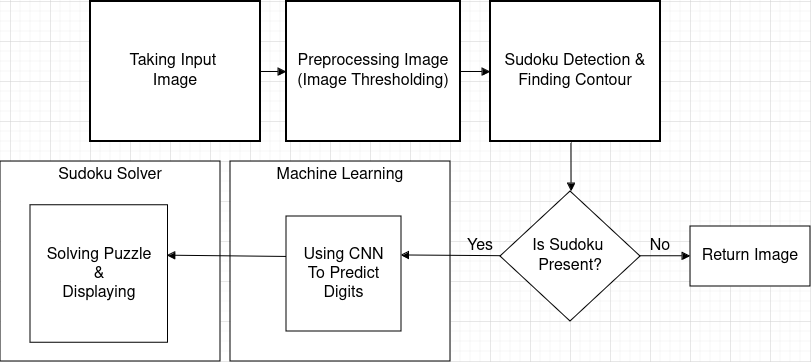
\includegraphics[scale=0.3]{assets/proposed_approach.png}}
\caption{The proposed approach}
\label{proposed_approach}
\end{figure}

\subsection{Preprocessing Image}\label{preprocess_step}
The OpenCV library is used to capture frames in real-time. Unlike the usual RGB format, the library reads images in BGR format. To simplify digit recognition, the image undergoes pre-processing before proceeding to the next part of the program. The image is first converted from BGR to GRAY format, and then Gaussian Blur and Adaptive Thresholding are applied to enhance the visibility of contours and text. This optimization facilitates the CNN model in accurately identifying the digits within the image. Moreover, it aids in the program's ability to easily detect the necessary contours to confirm the presence of a Sudoku puzzle in the image.

\begin{figure}[htbp]
\centerline{
    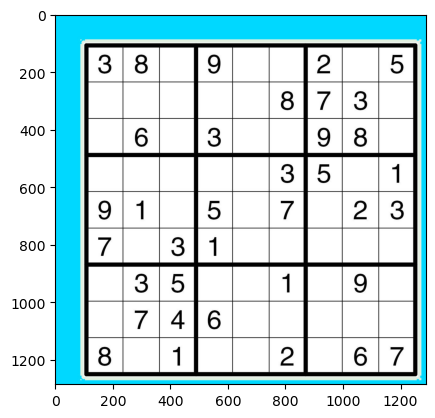
\includegraphics[scale=0.4]{assets/raw.png}
    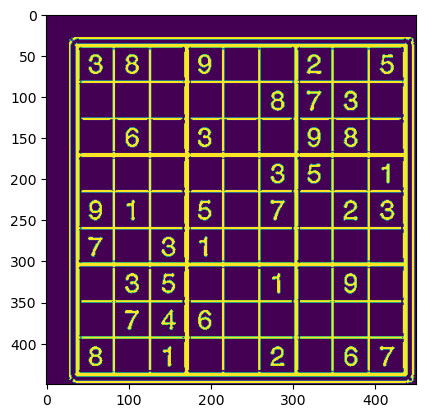
\includegraphics[scale=0.4]{assets/preprocess.png}
}
\caption{Raw image (left); Preprocessed image(right)}
\label{preprocessing_step}
\end{figure}

\subsection{Sudoku Detection}
To begin, the \verb|findContours| function from the cv2 library is utilized to locate and extract all contours present in the image. The largest contour found is then assumed to be the Sudoku puzzle. However, it is important to note that if there are any other significant contours in the image, they may be mistakenly identified as the Sudoku puzzle, leading to inaccurate results in certain scenarios. If no large contour is detected, the program will simply display the original image in the result window. Assuming a clear and visible Sudoku puzzle is present, the program proceeds to draw a virtual rectangle around the four corners of the puzzle. This step is crucial as it prepares the puzzle for further processing required to extract the data from it. If the image is captured from a different perspective or is angled differently, the \verb|warpPerspective| function is applied to warp the image into a frontal perspective. This transformation aids in digit recognition later on. Once the image has been warped, Gaussian blur and thresholding are applied again. The init grid is used to store the Sudoku board digits. The Sudoku board is then transformed into a 9 by 9 square grid, excluding the borders from processing to prevent the CNN model from mistakenly interpreting the gridlines as part of the digits. At this stage, only the numbers remain in the cropped image. To enhance their clarity and sharpness, binary thresholding is applied to the image. This further improves the visibility of the numbers for subsequent processing steps.

\begin{figure}[htbp]
\centerline{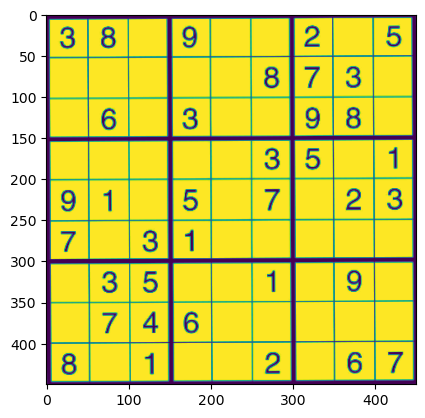
\includegraphics[scale=0.8]{assets/contour.png}}
\caption{The detected contour/sudoku puzzle.}
\label{contour_detection}
\end{figure}

\subsection{Sudoku reading using Machine Learning}
There are several methods available in programming to achieve digit recognition, but the most efficient and reliable approach is to use a Convolutional Neural Network (CNN) model. CNNs are commonly used for classification problems and are particularly effective for tasks like digit recognition and face recognition. The process of creating the model involves adding different layers such as convolution layer, flatten layer, max-pooling layer, dense layer, and dropout. The convolution layer plays a crucial role in extracting features from the input data. It establishes connections between these features and passes the output to the max-pooling layer, which reduces the dimension of the data to create an abstract representation of the input image. This abstract representation is further downsampled to extract more features. Dropout is used during model creation to deactivate a certain percentage of neurons in order to prevent overfitting. By doing so, the model becomes more adaptable to images with slight variations from the ones in the training set, rather than being limited to a specific type of image. The fully connected layer is responsible for connecting the extracted features with an activation function, which converts the array containing all the features into a 1-dimensional array. This array is then connected to a dense layer with 9 neurons, where each neuron represents a number from 1 to 9. 

\begin{figure}[htbp]
\centerline{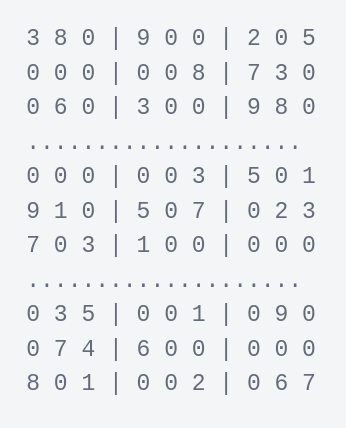
\includegraphics[scale=0.5]{assets/processed.png}}
\caption{The processed puzzle}
\label{processed_puzzle}
\end{figure}

The process of predicting the digits in a Sudoku puzzle is then accomplished using the predict function.

\subsection{Solving the Puzzle}\label{solving_puzzle}
The placement of the solution digit is determined by a backtracking algorithm that examines each empty cell and searches for a suitable digit placement.
\begin{figure}[htbp]
\centerline{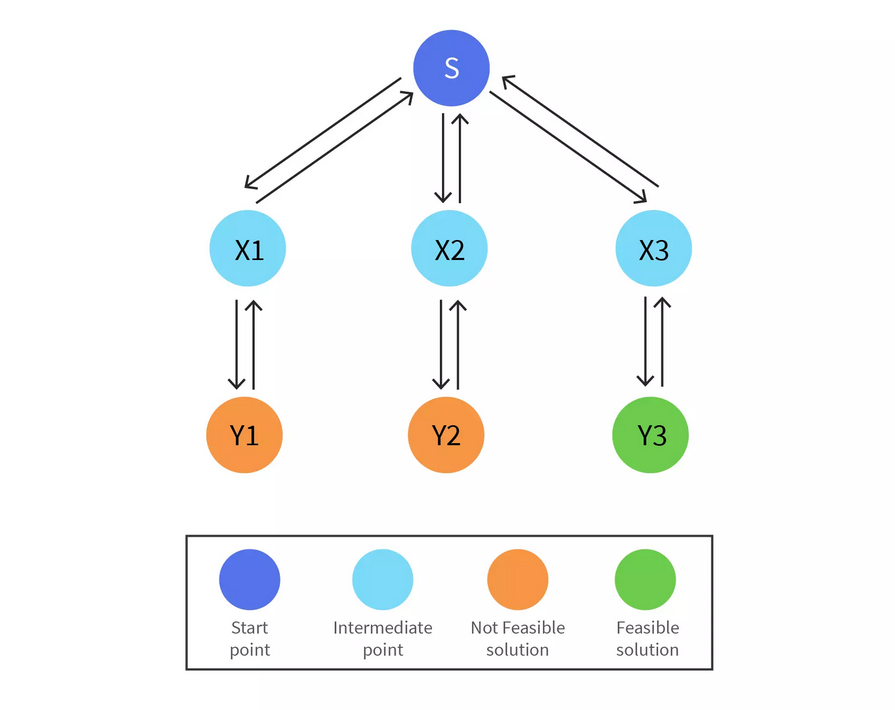
\includegraphics[scale=0.3]{assets/backtracking.png}}
\caption{Working of a backtracking algorithm}
\label{backtracking_algo}
\end{figure}

The algorithm starts by placing a digit in a cell and then checks all other cells in its row, column, and 3 by 3 region to ensure that the same digit does not already exist. If the digit is not found in the specified region, the algorithm moves on to the next cell. However, if the digit does exist in the specified cells, the algorithm clears the cell and tries another digit. This process continues until all cells are correctly filled. Before attempting to solve the Sudoku puzzle, the program verifies that it is not unsolvable. It does this by checking all possible positions in the array. Only after confirming the solvability does the program begin the solving process. The program constantly updates the array of digits based on the current state of the puzzle, allowing it to display the solution for the specific puzzle. It is worth noting that the program's performance and accuracy are not affected by switching between different Sudoku puzzles.


\subsection{Showing the Solution}
Once the solution array is populated, the website shows the result in the form of ASCII Monocode text, to make it look consistent. This is generated using the Python Flask project and HTMX, which takes solved sudoku returned from the Solving (\ref{solving_puzzle}) step, which is done using the recursive backtracking method \verb|solveSudokuPuzzle|. The solution which is returned is printed using \verb|printPuzzle|. The result is then shown in the browser inside a accordion which can be collapsed or expanded for easier viewing of the different sections.

\begin{figure}[htbp]
\centerline{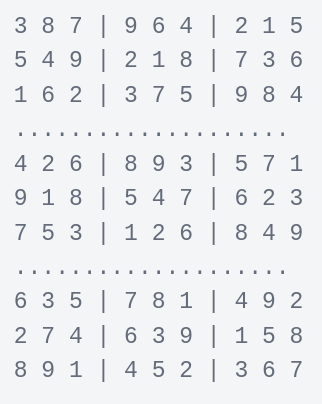
\includegraphics[scale=0.5]{assets/solved.png}}
\caption{The solved puzzle}
\label{solved_puzzle}
\end{figure}

\section{Results}
After training the model, we finally average around to an accuracy of 98\% for the training dataset as shown in Fig.~\ref{accuracy}. Given an input image, the loss-epoch graph can be seen in Fig.~\ref{loss_function}. Included below is a table (Table.~\ref{tab1}) showing the results from our various image testings.

\begin{figure}[htbp]
\centerline{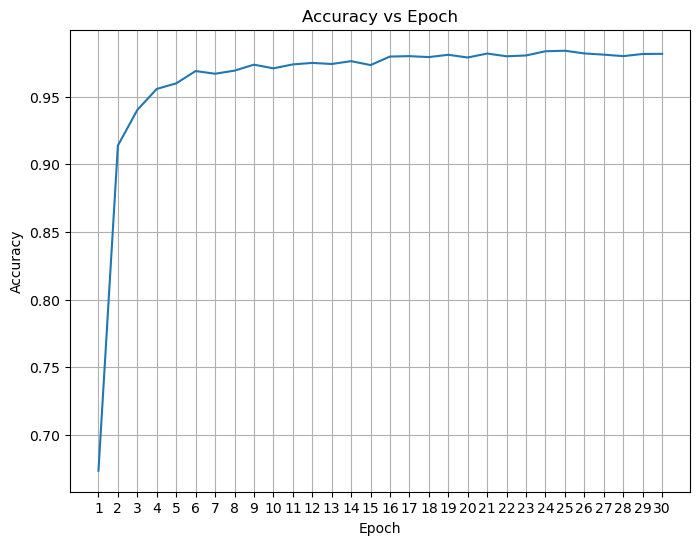
\includegraphics[scale=0.4]{assets/result-input/accuracy-over-epoch.png}}
\caption{Accuracy graph}
\label{accuracy}
\end{figure}

\begin{figure}[htbp]
\centerline{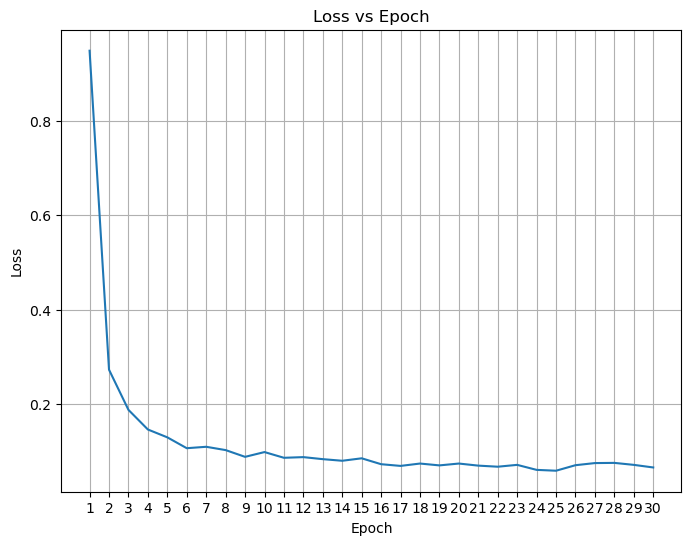
\includegraphics[scale=0.4]{assets/result-input/loss-over-epoch.png}}
\caption{Loss graph}
\label{loss_function}
\end{figure}

\begin{table}[htbp]
\caption{ACCURACY}
\begin{center}
\begin{tabular}{|c|c|c|c|c|}
\hline
S. No & No. of & Digits & Digits  & Sudoku \\
 & Digits & Correctly & Wrongly & Solved \\
 & & Identified & Identified & \\
\hline
& & & & \\
1 & 35 & 35 & 0 & Yes \\
& & & & \\
\hline
& & & & \\
2 & 35 & 35 & 0 & Yes \\
& & & & \\
\hline
& & & & \\
3 & 35 & 35 & 0 & Yes \\
& & & & \\
\hline
& & & & \\
4 & 35 & 35 & 0 & Yes \\
& & & & \\
\hline
& & & & \\
5 & 35 & 34 & 0 & Yes \\
& & & & \\
\hline
& & & & \\
6 & 26 & 26 & 0 & Yes \\
& & & & \\
\hline
& & & & \\
7 & 28 & 22 & 4 & No \\
& & & & \\
\hline
& & & & \\
8 & 28 & 25 & 0 & Yes \\
& & & & \\
\hline
& & & & \\
9 & 28 & 28 & 0 & Yes \\
& & & & \\
\hline
& & & & \\
10 & 35 & 35 & 0 & Yes \\
& & & & \\
\hline
& & & & \\
Total & 320 & 310 & & \\
& & & & \\
\hline
\end{tabular}
\label{tab1}
\end{center}
\end{table}

When you first run the application, it opens and shows up a local web server where you can upload the image of a sudoku from your camera or files, and then it'll show the various steps to get to our results. Different images were tested with this system with varying but satisfying results, and one such case is shown below from start to completion.

Fig.~\ref{input} is the default web page when we first run the app, and we can upload an input image, either from a camera or a locally selected file.

Fig.~\ref{generated_output} is the page after we have uploaded the input image, and it has finished processing it (shows a loading indicator otherwise). The page is divided into multiple sections, each showing a successive step towards the goal of reading and solving the Sudoku puzzle.

\begin{figure}[htbp]
\centerline{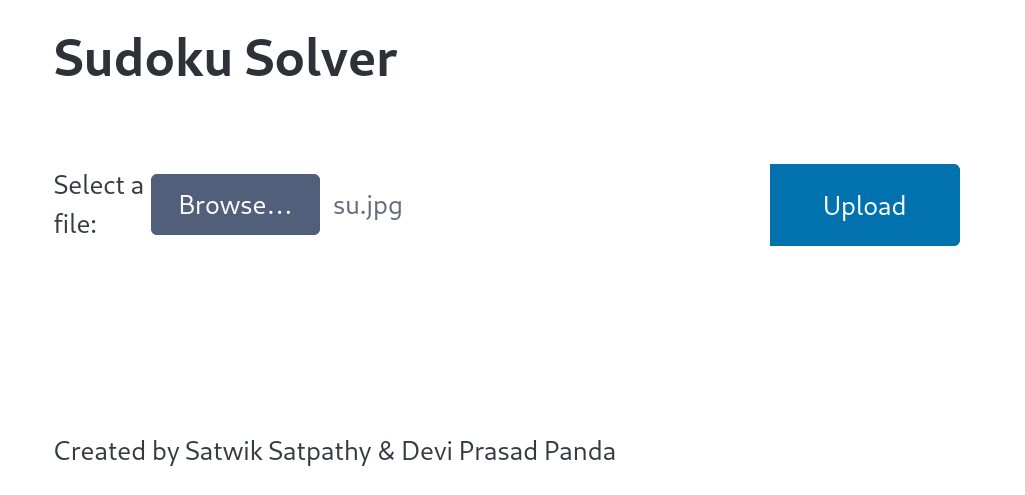
\includegraphics[scale=0.2]{assets/result-input/test1/1.png}}
\caption{Default look/Input}
\label{input}
\end{figure}

\begin{figure}[htbp]
\centerline{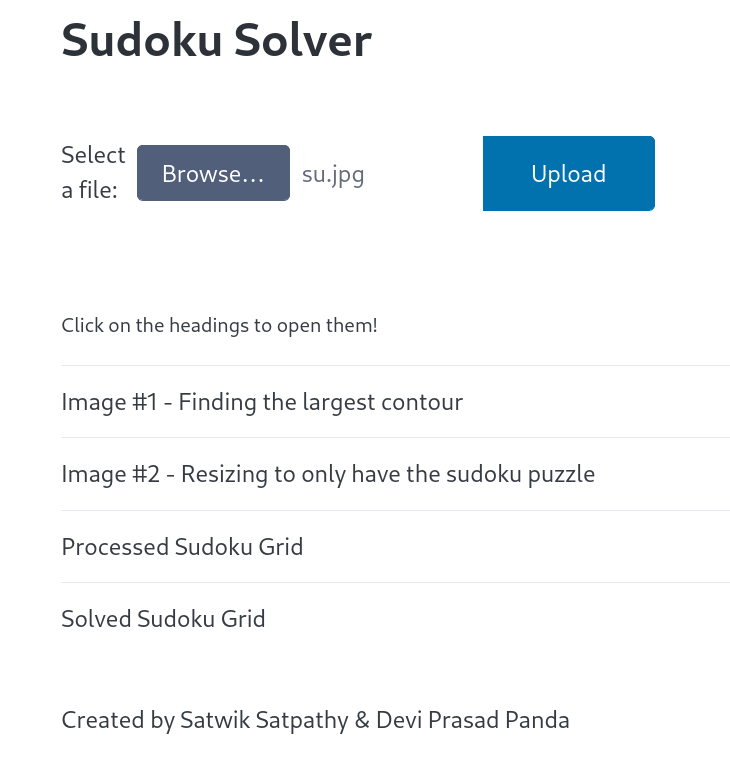
\includegraphics[scale=0.3]{assets/result-input/test1/3.png}}
\caption{Output Accordions Generated}
\label{generated_output}
\end{figure}

Finally, in Fig.~\ref{unsolved} and Fig.~\ref{solved}, we see the given input compared to the final output. All the digits are well placed within their boxes and the size of the digit is also matching with the size of the Sudoku. This indicates perfect
result with perfect output.

\begin{figure}[htbp]
\centerline{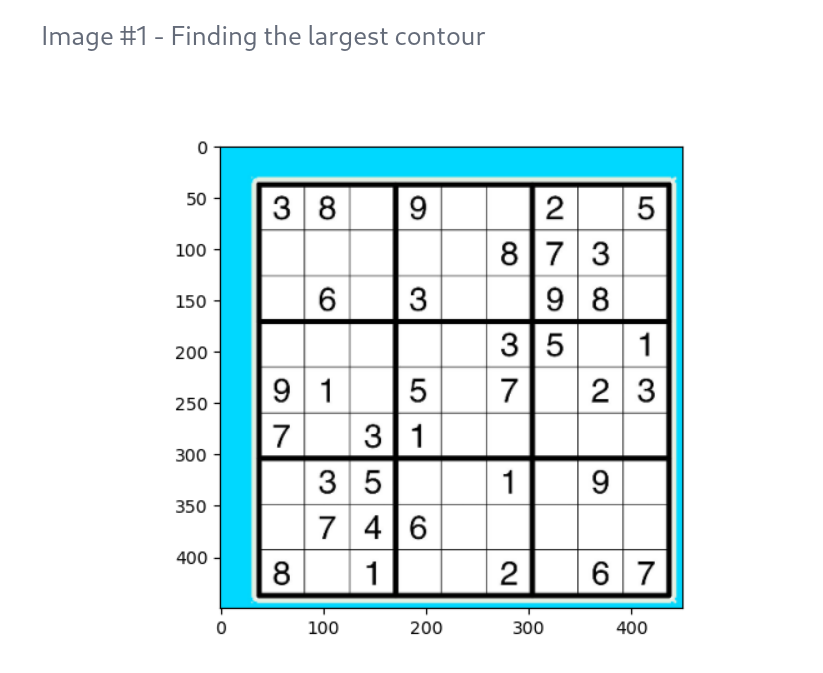
\includegraphics[scale=0.3]{assets/result-input/test1/4.png}}
\caption{Unsolved}
\label{unsolved}
\end{figure}

\begin{figure}[htbp]
\centerline{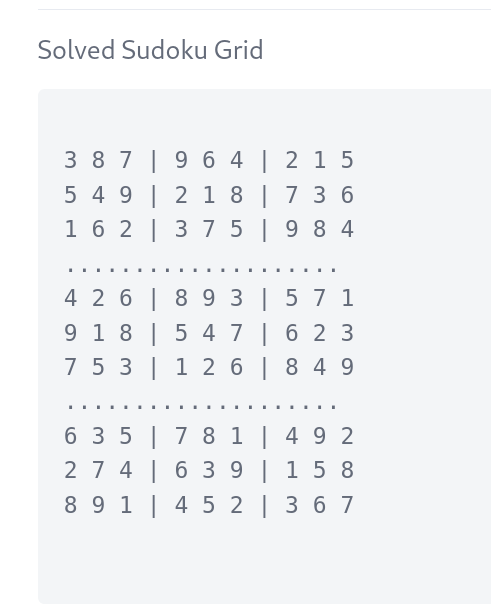
\includegraphics[scale=0.5]{assets/result-input/test1/7.png}}
\caption{Solved}
\label{solved}
\end{figure}

\section{Limitations}
The camera-based system used in this process relies on a high-quality camera to accurately detect the contours and digits in the image. If the image is blurry or of low quality, the results may be unclear. Additionally, proper lighting is crucial for the system to detect the Sudoku puzzle, which can take some time in certain situations. It is important for the image to be well aligned in order to avoid distortion caused by unreliable warping techniques. If the gridlines in the image are not clearly defined, the program may merge two cells into one, leading to conflicting results. While the numbers projected onto the image may be slightly off due to image quality issues, they will not overlap directly.

\section{Future Scope}
This comprehensive package is designed for effortless installation on desktops or laptops, or as a website available through the cloud, making it accessible to all users. Further enhancements to the algorithm will streamline the Sudoku-solving process, minimizing technical demands. Integration of pre-trained models for digit recognition will not only boost accuracy but also lessen the need for extensive computational capabilities.

\section{Conclusion}
We have thoroughly examined all the components necessary to create a Sudoku solver that is both effective and dependable by utilizing various programming language techniques. We explored the different stages involved in ensuring the program's success, starting with preprocessing the input image through thresholding and gaussian blur before moving on to the task of identifying the Sudoku puzzle within the image. Once the Sudoku is detected, a CNN model is utilized to identify and record the digits present in the grid, storing them in an array. The backtracking algorithm is then implemented to fill in the empty spaces of the array with unique digits in each row, column, and 3 by 3 cell region, adhering to the rules of the Sudoku game. The result is then sent to the client and is displayed with various steps there.

\begin{thebibliography}{00}
\bibitem{b1} Ballard, D.H. (1982). CM Brown Computer Vision. NY: Prentice Hill
\bibitem{b2} Dutta, A., \& Ghosh, A. (2016, October). Development of a character recognition software to solve a Sudoku puzzle. In Information Technology, Electronics and Mobile Communication Conference (IEMCON), 2016 IEEE 7th Annual (pp. 1-5). IEEE.
\bibitem{b3} Simha, P. J., Suraj, K. V., \& Ahobala, T. (2012, March). Recognition of numbers and position using image processing techniques for solving sudoku puzzles. In Advances in Engineering, Science and Management (ICAESM), 2012 International Conference on (pp. 1-5). IEEE.
\bibitem{b4} Russell, E., \& Jarvis, F. (2006). Mathematics of Sudoku II. Mathematical Spectrum, 39(2), 54-58.
\bibitem{b5} Douglas, D. H., \& Peucker, T. K. (1973). Algorithms for the reduction of the number of points required to represent a digitized line or its caricature. Cartographica: The International Journal for Geographic Information and Geovisualization, 10(2), 112-122.
\bibitem{b6} Manav B. Sanghavi, Aniket K. Rupani, Mahek S. Maniar, Sai Deepthi Pabba, “Solving Sudoku from an Image using Modular Architecture Approach”, International Journal on Recent and Innovation Trends in Computing and Communication , Volume: 3 Issue: 3, March 2015
\bibitem{b7} ARNAB K. MAJI, SUDIPTA ROY, RAJAT K. PAL , “A Novel Algorithmic approach for solving Sudoku puzzle in Guessed Free Manner”, EUROPEAN ACADEMIC RESEARCH, VOL. I, ISSUE 6/SEPEMBER 2013
\bibitem{b8} Akash Dutta , Arunabha Ghosh , “Development of a Character Recognition Software to solve a Sudoku Puzzle”, IEEE 2016
\bibitem{b9} Mrs. Supriya H.S, Ayush Baran, Processing Sudoku Images and Solving
by Recursive Backtracking Algorithm, International Journal for
Scientific Research \& Development| Vol. 5, Issue 04, 2017 | ISSN
(online): 2321-0613
\bibitem{b10} Shin, Hoo-Chang, et al. "Deep convolutional neural networks for
computer-aided detection: CNN architectures, dataset characteristics and
transfer learning." IEEE transactions on medical imaging 35.5 (2016):
1285-1298.
\bibitem{b11} Dhanya Job and Varghese Paul. Recursive backtracking for solving 9*9
sudoku puzzle. 2016.
\bibitem{b12} Heimo, O.I., Kimppa, K.K., Helle, S., Korkalainen, T., Lehtonen, T.:
Augmented reality - towards an ethical fantasy? In: 2014 IEEE Interna-
tional Symposium on Ethics in Science, Technology and Engineering,
pp. 1– 7, 23–24 May 2014
\end{thebibliography}

\end{document}
